\documentclass[10pt, aspectratio=169]{beamer}
\usepackage{caption}
\usepackage{subcaption}
\usetheme[progressbar=frametitle]{metropolis}
\usepackage{amsmath}
\usepackage{siunitx}
\usepackage{xcolor}
\usecolortheme{crane}
\definecolor{craneorange}{rgb}{0.53,0.66,0.42}
\usecolortheme{spruce}
\usepackage{hyperref}
\usepackage{multimedia}
\usepackage[percent]{overpic}
\usepackage[para]{footmisc}

\title{Computational study of far-field acoustic emission by collapsing bubbles}
\date{\today}
\author[shortname]{Magu Raam Prasaad R}
\institute[shortinst]{Indian Institute of Science, Bangalore}

\begin{document}
\begin{frame}
	\maketitle
\end{frame}

\begin{frame}{Introduction}
	\begin{columns}
		\column{0.5\textwidth}
		\begin{itemize}
			\item High-speed flows lead to the formation of cavitation bubbles.
			\item Collapsing cavitation bubbles form blast and shock waves.
			\item Blast wave emission process are the strong source of acoustic waves.
		\end{itemize}
				
		\column{0.5\textwidth}
		\begin{figure}[h]
			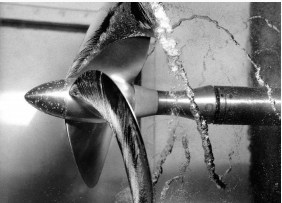
\includegraphics[scale = 0.55]{images/propeller.png}
			\caption{Cavitation bubbles around rotating propeller\cite{propeller}}	
		\end{figure}
							
	\end{columns}
	\footnotetext[1]{Brennen C. E, JFM 2002}
\end{frame}

\begin{frame}{Computational approach}
	
	\begin{itemize}
		\item In this work we compute the far-field acoustic waves emitted from bubble collapse process using the Kirchhoff integral formulation.
	\end{itemize}

	\begin{figure}
		\centering
		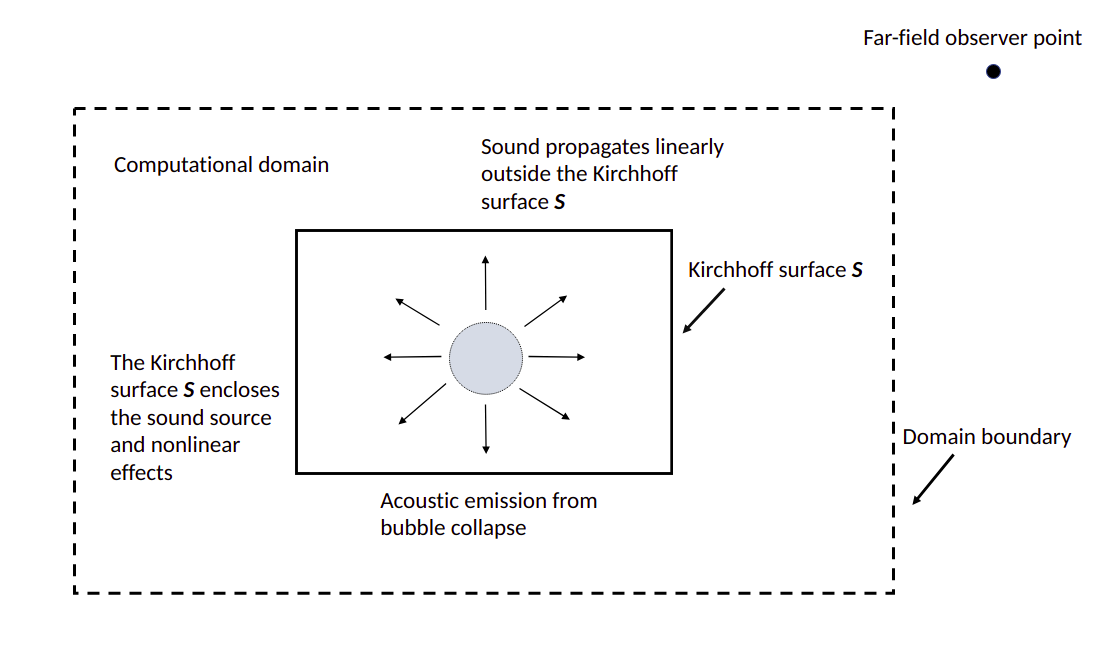
\includegraphics[scale=0.22]{images/shematic1.png}
		\caption{Schematic of far-field acoustic data computed from CFD solver using the Kirchhoff integral method.}
	\end{figure}		

\end{frame}

\begin{frame}{Kirchhoff integral formulation}
	\begin{columns}
		\column{0.5\textwidth}
		\begin{itemize}
			\item We chose a control surface $S$ that encloses all the acoustic sources, and the pressure perturbations $p'$ satisfies the homogeneous wave equation.
			\begin{equation}\label{Wave equation}
				\Bigg( \frac{1}{c_{0}^2}\frac{\partial{}^{2}}{\partial{t}^{2}}- \nabla{}^{2} \Bigg) p' = 0 \quad \quad \textrm{in} \ V.
			\end{equation}
			\item The control surface S is defined by $f(\mathbf{x}) = 0$, $f(\mathbf{x}) > 0$ for $\mathbf{x}$ in V and $f(\mathbf{x}) < 0$ for $\mathbf{x}$ inside surface S.
		\end{itemize}
				
		\column{0.5\textwidth}
		\begin{figure}[h]
			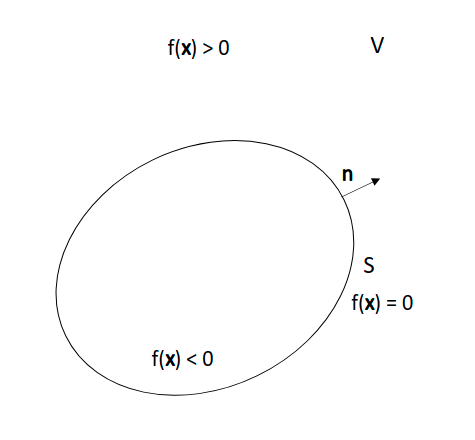
\includegraphics[scale = 0.3]{images/kirchhoff_surface.png}
			\caption{Stationary Kirchhoff surface $S$ encloses sound source}	
		\end{figure}
							
	\end{columns}
\end{frame}

\begin{frame}{Kirchhoff integral formulation}
	\begin{columns}
		\column{0.5\textwidth}
		\begin{itemize}
			\item We define the pressure $p'$ as a generalized function $pH(f)$ where
			\begin{equation*}\label{Generalized_Functions}
				p' H(f) =\begin{cases}
					p' , & \text{for $\mathbf{x}$ in V}.     \\
					0,  & \text{for $\mathbf{x}$ inside S}.
				\end{cases}
			\end{equation*}
			\item The acoustic wave equation in generalised pressure
			\begin{equation*}\label{Generalized Wave Equation}
				\Bigg( \frac{1}{c_{0}^2}\frac{\partial{}^{2}}{\partial{t}^{2}}- \nabla{}^{2} \Bigg) p'H = -\frac{\partial p'}{\partial n}\delta(f) - \nabla.(p' \mathbf{n} \delta(f)).
			\end{equation*}
		\end{itemize}
				
		\column{0.5\textwidth}
		\begin{figure}[h]
			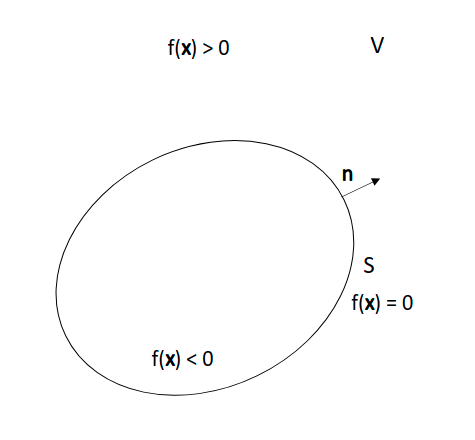
\includegraphics[scale = 0.3]{images/kirchhoff_surface.png}
			\caption{Stationary Kirchhoff surface $S$ encloses sound source}	
		\end{figure}
							
	\end{columns}
\end{frame}

\begin{frame}{Kirchhoff integral formulation}
	\begin{itemize}
		\item The acoustic wave equation in generalized variables is valid in the
		entire unbounded space. Therefore we can use the free-space Green’s function to
		solve the equation.
		\begin{equation}\label{pressure}
			p'(\mathbf{x}, t) = \int s(\mathbf{y}, \tau){G(\mathbf{x}, t; \mathbf{y}, \tau )} d\mathbf{y}d\tau.
		\end{equation}
		where,
		\begin{equation}\label{Green's Function}
			G(\mathbf{x}, t; \mathbf{y}, \tau ) = \frac{\delta \Big(t - \tau - \frac{|\mathbf{x} - \mathbf{y}|}{c_{0}}\Big)}{4\pi|\mathbf{x} - \mathbf{y}|}
		\end{equation}
		and 
		\begin{equation}
			s(\mathbf{y}, \tau) = -\frac{\partial p'}{\partial n}\delta(f) - \nabla.(p' \mathbf{n} \delta(f)).
		\end{equation}
	\end{itemize}
\end{frame}

\begin{frame}{Kirchhoff integral formulation}
	\begin{itemize}
		\item Simplifying the equation further, we obtain the Kirchhoff integral equation for a stationary control surface
		\begin{equation}
			\begin{split}
				p'(\mathbf{x}, t) = -\frac{1}{4\pi}\int_{S}\Big[  \frac{p'}{r^{2}}\frac{\partial r}{\partial n} - \frac{1}{r}\frac{\partial p'}{\partial n} + \frac{1}{c r}\frac{\partial r}{\partial n}\frac{\partial p'}{\partial \tau} \Big]_{\tau} dS.
			\end{split} 
		\end{equation}
		$p'$ is the acoustic pressure satisfying the wave equation outside the control surface \textbf{S}, $c$ is the speed of sound at ambient conditions and $n$ is the normal.
		The integrands are evaluated at the emission time $\tau = t - \mathbf{r}/c$ and $\mathbf{r}= |\mathbf{x} - \mathbf{y}|$ is the distance between observer and source.
		\item The $p'$, ${\partial p'}/{\partial t}$ and ${\partial p'}/{\partial n}$ are computed from flow solver.
	\end{itemize}
\end{frame}

\begin{frame}{Axisymmetric test case - Cylindrical wave}
	\begin{itemize}
		\item The axisymmetric acoustic wave equation in a cylindrical coordinate system, assuming cylindrical wave solution, $\partial p'/\partial \theta = 0$ and $\partial p'/\partial z = 0$
		\begin{equation}\label{Cylindrical wave equation}
			\Bigg( \frac{1}{c^2}\frac{\partial{}^{2}}{\partial{t}^{2}}- \frac{\partial^2}{\partial r^2} - \frac{1}{r}\frac{\partial}{\partial r}  \Bigg) p' = 0.
		\end{equation}
		\item Substituting $p'(r, t) = R(r)e^{i\omega t}$ in the wave equation we obtain
		\begin{equation}
			\frac{d^2 R}{dr^2} + \frac{1}{r}\frac{dR}{dr} + k^2R = 0.
		\end{equation}
		\item Where $k^2 = {\omega^2}/{c^2}$. The general solution of equation is given by Hankel function
		\begin{equation}
			p'(r, t) = AH_{0}^{(1)}(kr)e^{i\omega t}.
		\end{equation}
	\end{itemize}
\end{frame}

\begin{frame}{Axisymmetric test case - Cylindrical wave}
	\begin{itemize}
		\item The solution $p'(r, t) = AH_{0}^{(1)}(kr)e^{i\omega t}$ is singular at $r = 0$. 
		\item For $r \to 0 $ The function has a logarithmic singularity
		\begin{equation}
			p'(r, t) \cong (2i A/\pi)\log(k r)e^{-i\omega t}.
		\end{equation}
	\end{itemize}
\end{frame}


\begin{frame}{Axisymmetric test case - Cylindrical wave}
	\begin{itemize}
		\item We use the cylindrical wave solution $p'(r, t) = AH_{0}^2(kr)e^{i\omega t}$ to validate the Kirchhoff solver.
		\item Where the amplitude, wave number and angular frequency are $A = 1.0, k = 1.0, \omega = 1.0$.
		\begin{figure}
			\centering
			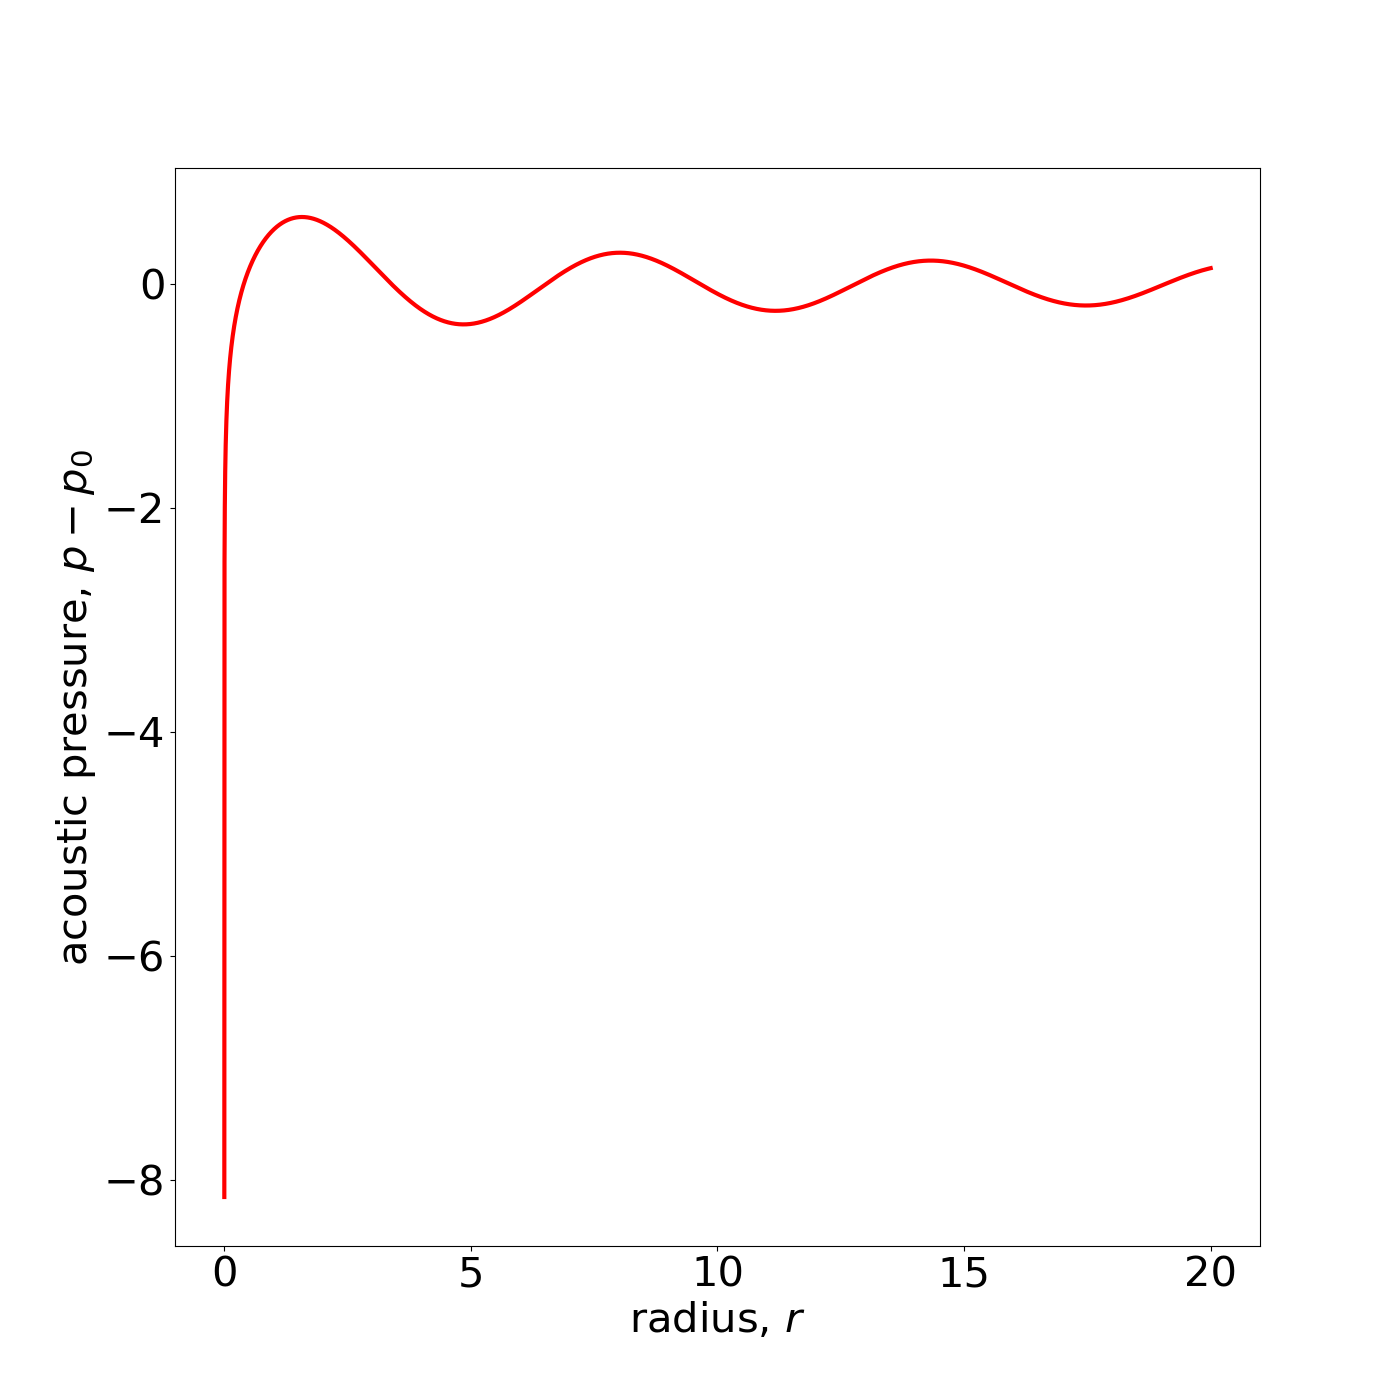
\includegraphics[scale=0.15]{images/cylindrical.png}
			\caption{Cylindrical wave solution at $t = 0.0$. The solution is singular at $r = 0.0$}
		\end{figure}
	\end{itemize}
\end{frame}

\begin{frame}{Axisymmetric test case}
	\begin{figure}
		\centering
		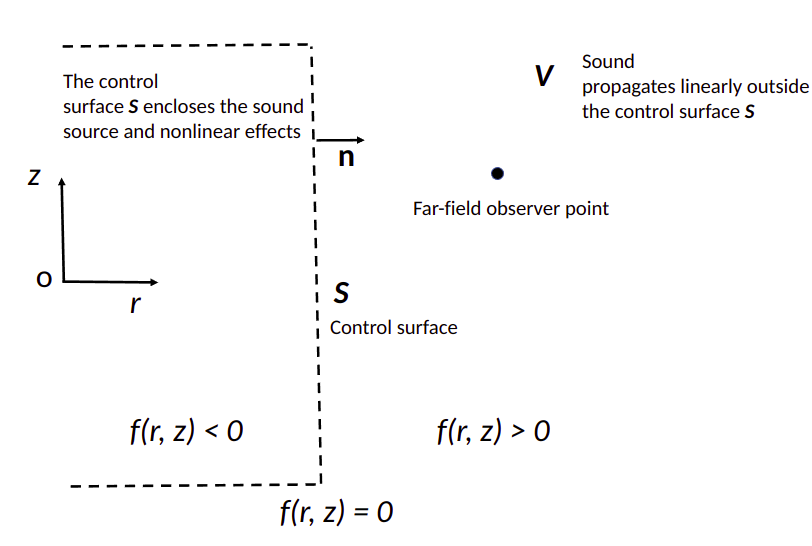
\includegraphics[scale=0.3]{images/shematic2.png}
		\caption{Axisymmetric Kirchhoff surface}
	\end{figure}

\end{frame}


\begin{frame}{Kirchhoff integral on a cylinder}
	\begin{figure}
		\centering
		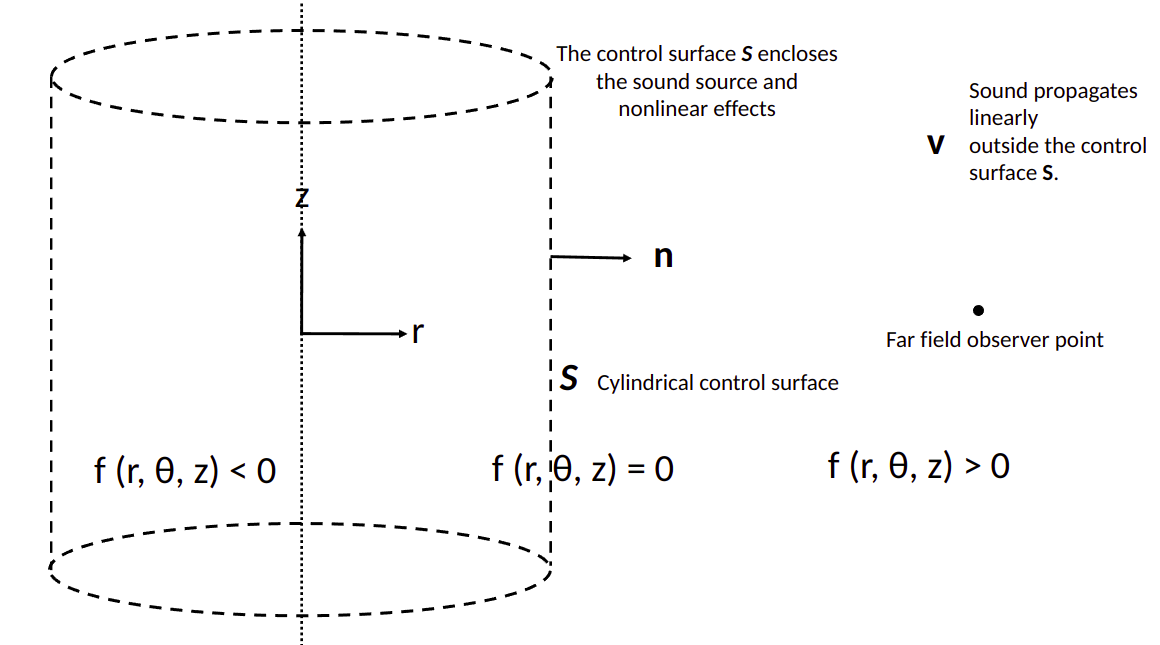
\includegraphics[scale=0.24]{images/cylinder.png}
		\caption{Cylindrical Kirchhoff surface}
	\end{figure}
\end{frame}

\begin{frame}{Kirchhoff integral on a cylinder}
	\begin{itemize}
		\item We compute the Kirchhoff integral on a cylindrical surface 
		\begin{equation}
			\begin{split}
				p'(r', z', t) =  -\frac{1}{4\pi}\int_{S_{top, bottom}}\Big[  \frac{p'}{r^{2}}&\frac{\partial r}{\partial n} - \frac{1}{r}\frac{\partial p'}{\partial n} + \frac{1}{c r}\frac{\partial r}{\partial n}\frac{\partial p'}{\partial \tau} \Big]_{\tau} r'dr'd\theta' \\
								 -\frac{1}{4\pi}\int_{S_{curved}} \Big[  \frac{p'}{r^{2}}&\frac{\partial r}{\partial n} - \frac{1}{r}\frac{\partial p'}{\partial n} + \frac{1}{c r}\frac{\partial r}{\partial n}\frac{\partial p'}{\partial \tau} \Big]_{\tau} Rd\theta'dz'  
			\end{split} 
		\end{equation}
		\item The above integral is numerically computed using Gauss quadrature
		\begin{equation}
			\begin{split}
				p'(r', z', t) =  -\frac{1}{4\pi}\sum_{i}^{N_r}\sum_{j}^{N_\theta}\sum_q^{Nqpts} \Big[  \frac{p'}{r^{2}}&\frac{\partial r}{\partial n} - \frac{1}{r}\frac{\partial p'}{\partial n} + \frac{1}{c r}\frac{\partial r}{\partial n}\frac{\partial p'}{\partial \tau} \Big]_{\tau} r'\Big |_q J_q w_q\\
								 -\frac{1}{4\pi}\sum_{j}^{N_\theta}\sum_{k}^{N_z}\sum_q^{Nqpts} \Big[  \frac{p'}{r^{2}}&\frac{\partial r}{\partial n} - \frac{1}{r}\frac{\partial p'}{\partial n} + \frac{1}{c r}\frac{\partial r}{\partial n}\frac{\partial p'}{\partial \tau} \Big]_{\tau} R \Big |_q J_q w_q 
			\end{split} 
		\end{equation}
		\item We use two-point Gauss quadrature on a reference cell $[-1, 1]\times [-1, 1]$. The quadrature points are mapped to computational cell using bi-linear interpolation. 
	\end{itemize}
\end{frame}

\begin{frame}{Kirchhoff integral on a cylinder}

	\begin{figure}
		\centering
		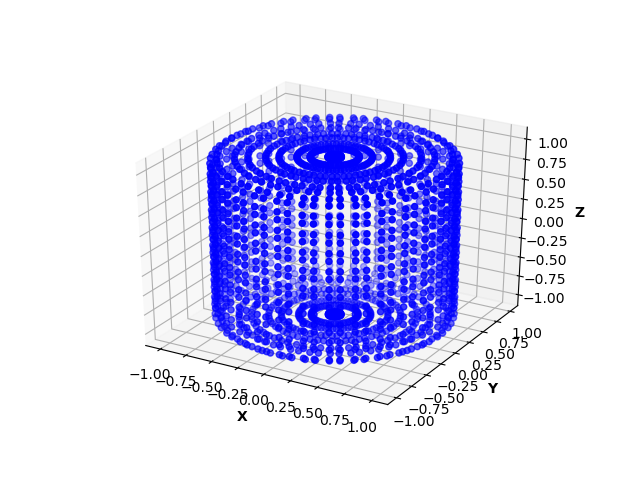
\includegraphics[scale=0.5]{images/quadpoints.png}
		\caption{Schematic of quadrature points on cylindrical surface}
	\end{figure}
\end{frame}


\begin{frame}{Results - Cylindrical wave}
	\begin{figure}
		\centering
		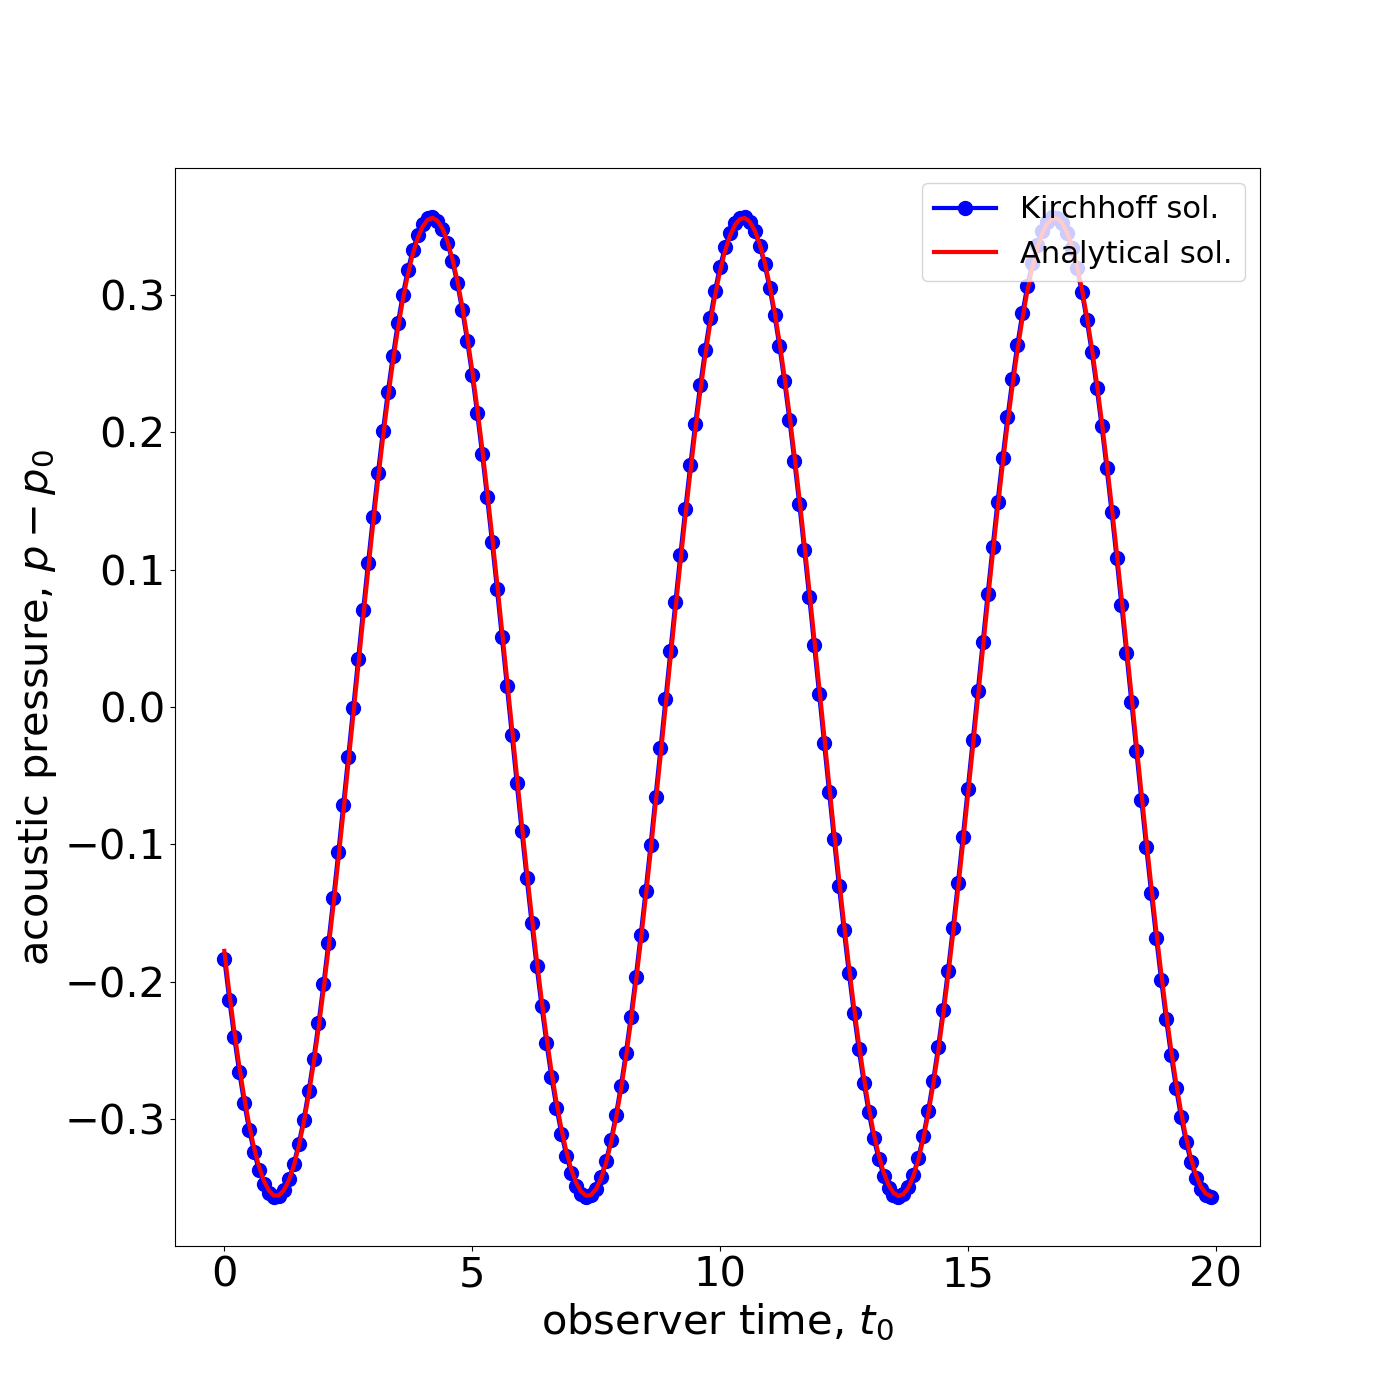
\includegraphics[scale=0.15]{images/Hankel.png}
		\caption{Acoustic pressure is computed at observer point ($r_{0}, \theta_{0}, z_{0}$) $= (5.0, 0, 0)$ using the Kirchhoff method and compared with the analytical solution. We chose a cylinder of radius $R = 0.5$ and height $H = 200$ centered at origin and $dr = d\theta = dz = 0.1$.}
	\end{figure}
\end{frame}

\begin{frame}{Results - Cylindrical wave}
	\begin{figure}
		\centering
		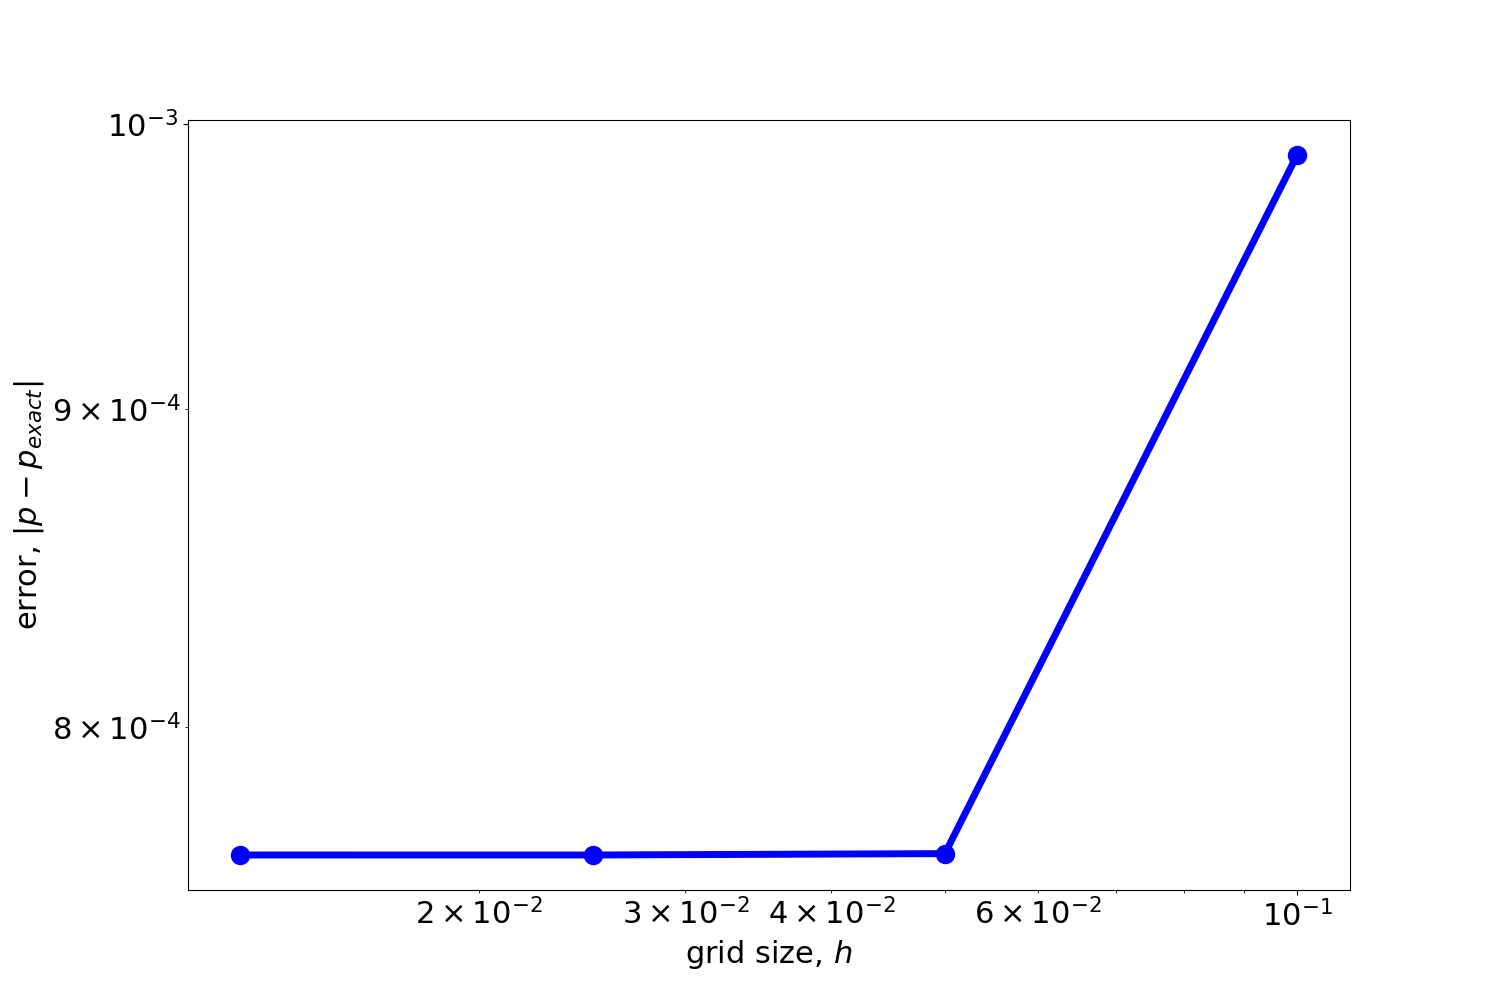
\includegraphics[scale=0.25]{images/convergence.png}
		\caption{Convergence of Kirchhoff integral.}
	\end{figure}
\end{frame}

\begin{frame}{Three dimensional test case - Acoustic monopole}
	\begin{itemize}
		\item We solve the acoustic wave equation
		\begin{equation}
			\Bigg( \frac{1}{c_{0}^2}\frac{\partial{}^{2}}{\partial{t}^{2}}- \nabla{}^{2} \Bigg) p'(\mathbf{x}, t)  = -q(t)\delta(\mathbf{x}), 
		\end{equation}
		for a monopole source using the \textbf{Kirchhoff} method.
		\item And compare it with the exact solution $p'(\mathbf{x}, t) = -\frac{1}{4\pi} \frac{  q(t - \frac{r}{c_{0}}) }{r}$.
		\item We chose a monopole source
		\begin{equation}
			q(t) = 2(t - t0)f_{0}^{2}\exp( -f_{0}^2(t - t_{0})^{2}), 
		\end{equation}
		where $f_{0} = 100$ is the dominant frequency and $t_{0} = \frac{4}{f_{0}}$.
	\end{itemize}
\end{frame}


\begin{frame}{Three dimensional test case - Acoustic monopole}
	\begin{itemize}
		\item We discretize a cuboidal domain of size $[-5.0,5.0]\times[-5.0,5.0]\times[-5.0,5.0]$ using $200 \times 200 \times 200$ cells.
		\item We enclose the monopole source using a cuboidal Kirchhoff surface whose diagonally opposite points are $p_{1} = (-1.0, -1.0, -1.0)$
		and $p_{2} = (1.0, 1.0, 1.0)$.
		\item The Kirchhoff surface is discretized into square cells of size $h = 0.1$.
		\item We store the analytical pressure at cell centers and interpolate it to the Kirchhoff surface using the fourth-order WENO polynomial.
		\item We interpolate the pressure data at emission time using the Linear polynomial.
		\item The Kirchhoff Integral is computed using the two-point Gauss quadrature formula.
	\end{itemize}
\end{frame}

\begin{frame}{Results - Acoustic monopole}
	\begin{figure}
		\centering
		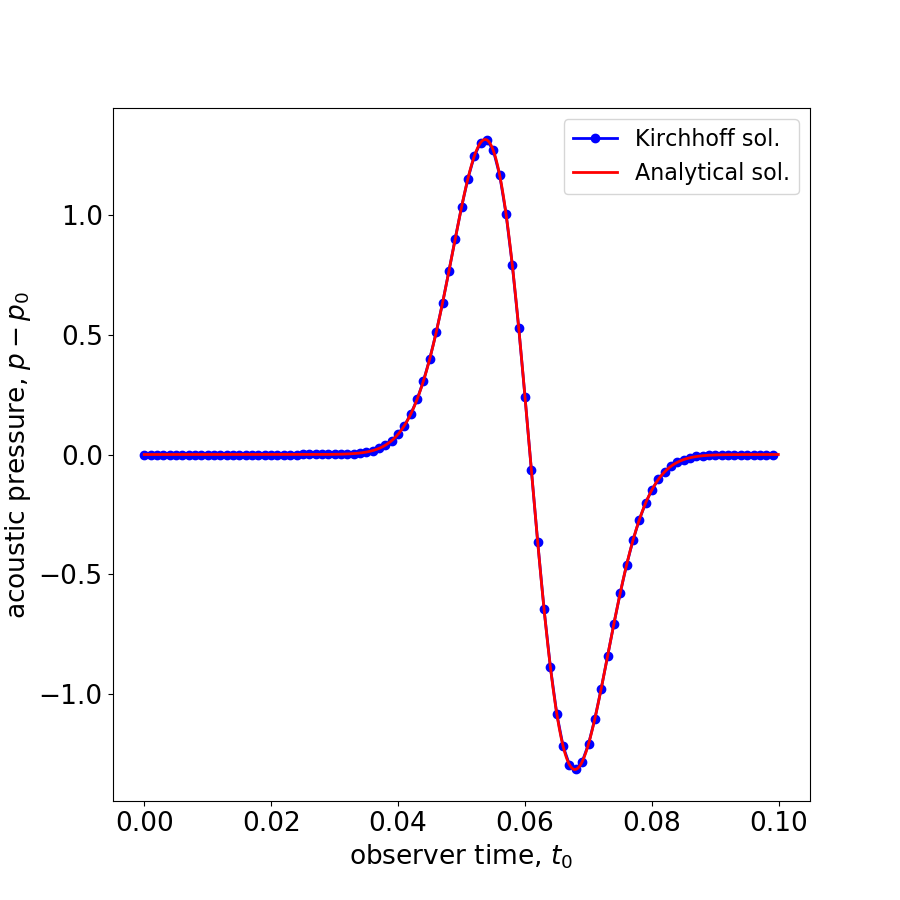
\includegraphics[scale=0.26]{images/monopole.png}
		\caption{Acoustic pressure is computed at observer point $x_{0} = (3, 3, 3)$ using the Kirchhoff method and compared with the analytical solution.}
	\end{figure}
\end{frame}

\begin{frame}{Conclusion}
	\begin{itemize}
		\item We have written a Kirchhoff solver to compute the far-field pressure from CFD data.
		\item We have tested our solver with analytical solution for axisymmetric and three-dimensional wave equation.
	\end{itemize}
	Future work:
	\begin{itemize}
		\item To compute the far-field acoustic waves emitted from axisymmetric bubble collapse
			  using the developed Kirchhoff solver. 
	\end{itemize}
\end{frame}

\begin{frame}[allowframebreaks]{Bibliography}
	\frametitle{Bibliography}
	\bibliographystyle{amsplain}
	\begin{thebibliography}{99}
		\bibitem{propeller} Duttweiler M. E., Brennen C. E. Surge instability on a cavitating propeller [J]. Journal of Fluid Mechanics, 2002, 458: 133-152.
		
	\end{thebibliography}
\end{frame}

\begin{frame}[standout]
	Thank you!
\end{frame}
\end{document}